\part{Explication des méthodes utilisées}
\chapter{}
\section{Presentation}
Afin de préparer mon travail de M2 et établir une base de référence des données quantitatives, la première étape de ma méthodologie consiste au traitement de la base de données des « Militaires décédés sur les théâtres d'opérations extérieurs (1905-1962) ».  Ensuite je pourrais concevoir un échantillon représentatif de fiches matricules et procéder à une transcription et extraction des données. L’étape finale de la méthodologie serait de vérifier les données présentes avec l’information nichée dans le JMOs pour éviter d'éventuelles analyses anachroniques et essentielles qui pourraient être liées aux méthodes quantitatives. Cette section de mon rapport présentera l'extraction de ma base de données et un aperçu de mes méthodes potentielles pour le traitement des registres matricules. 
\begin{figure}[H]
    \centering
    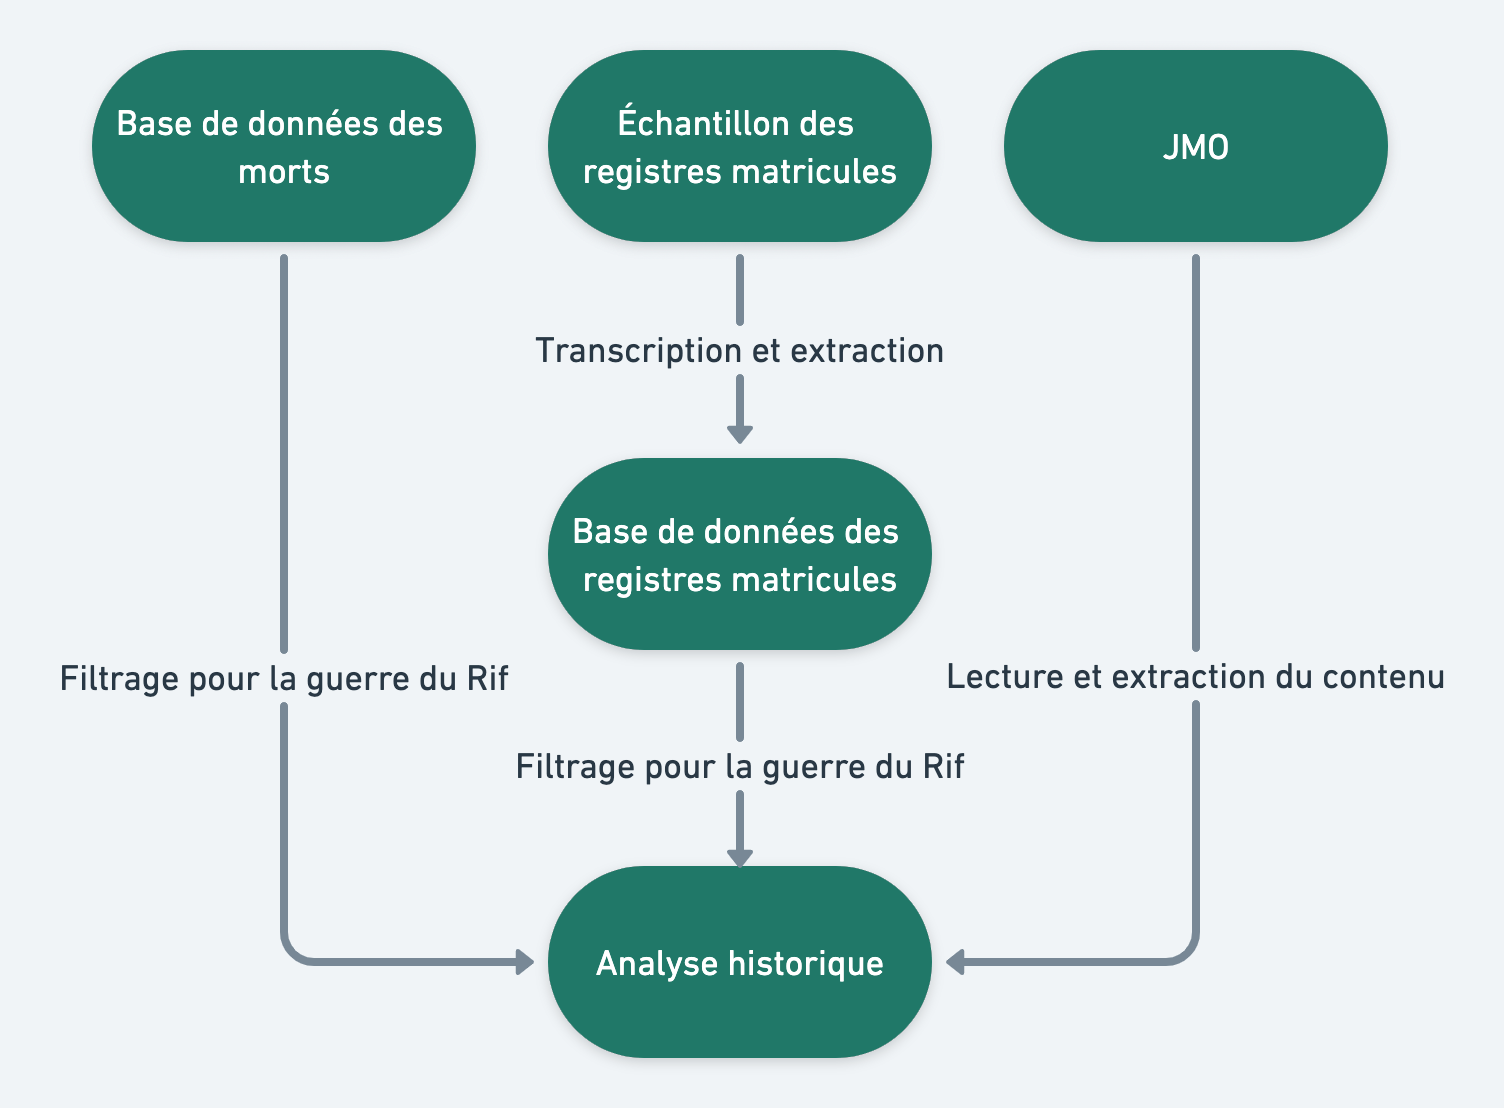
\includegraphics[scale=0.25]{Images/pipeline.png}
    \caption{Organigramme de la méthode}
    \label{fig:Pipeline}
\end{figure}
Enfin, je voudrais attirer l'attention sur un détail que je n'ai pas oublié : les historiens doivent être très prudents lorsqu'ils interprètent des données quantitatives comme une réalité de ce qu'était le passé. De nombreuses études et débats historiographiques ont démontré que la qualité la plus importante pour l'historien quantitatif est l'humilité. Je crois que la méthodologie reflète cette aspiration.

\section{Nettoyage de la base}
Grâce à la disponibilité au format csv de la base de données des morts en opération extérieure, je n'ai pas eu besoin de faire un scrapping du site du SHD. J'ai téléchargé l’intégralité des données directement de ce lien. J'ai ensuite procédé au traitement de la  base « Militaires décédés sur les théâtres d'opérations extérieurs (1905-1962) » avec la librairie \textbf{Pandas} de \textbf{Python}. Après  j'ai filtré la base de données par année et par lieu de décès. La période qui m'intéresse va de janvier 1925 à décembre 1926, la période pendant laquelle la majorité des combats ont eu lieu. Dans la base de données, il y a une colonne pour le pays de décès à partir de laquelle j'ai filtré pour le Maroc. Le script que j'ai utilisé pour filtrer la base de données se trouve sur la \textbf{branch master} dans le dossier \textbf{dbCreation} de mon projet sur \href{https://github.com/the0phil3/projetMemoire}{Github}. Ce travail m'a permis de créer une base de données personnelle des sujets qui m'intéressent.
\begin{figure}[H]
    \centering
    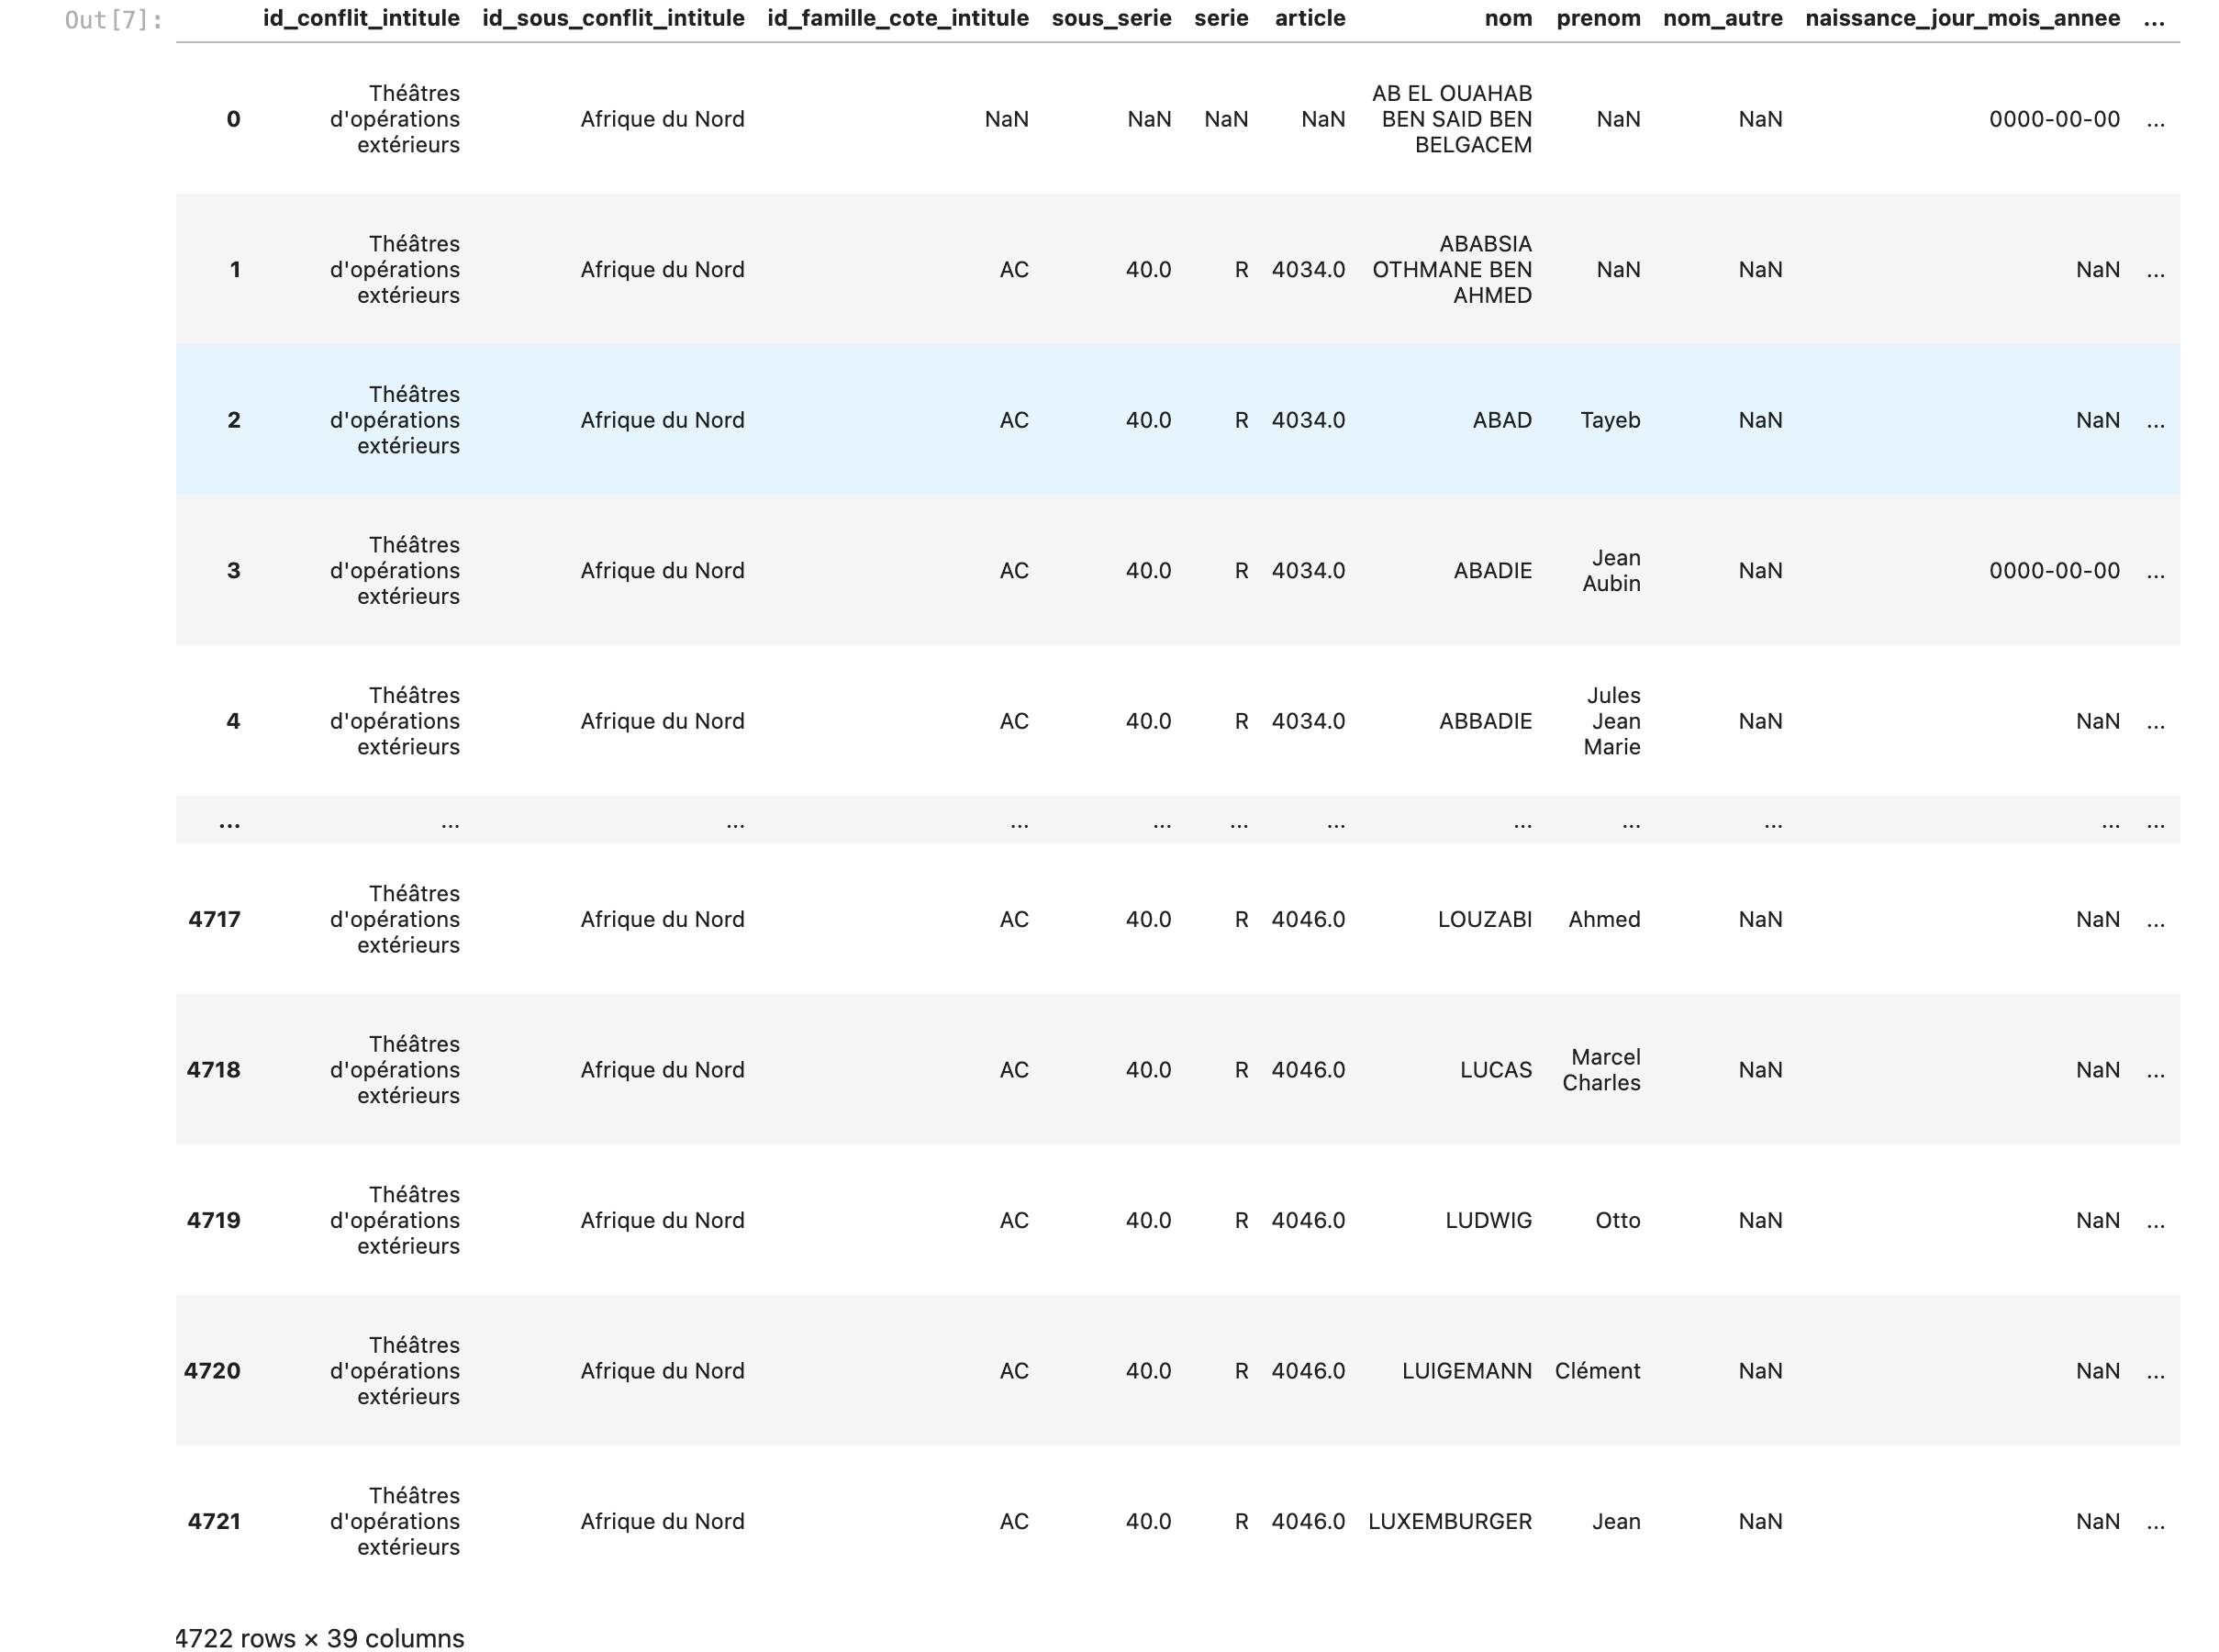
\includegraphics[scale=0.3]{Images/mortsduRif.png}
    \caption{Base de données traitée}
    \label{fig:Base de données}
\end{figure}
Lors de mon premier traitement de cette base de données, j'ai eu comme difficultés que j'ai pu résoudre: \begin{enumerate}
\item Trouver l'origine des données chiffrés 
\item Enlever les doubles des soldats
\item Rendre lisible les dates par \textbf{Pandas}   
\end{enumerate}

L’information disponible sur le site \underline{Mémoire des hommes} au sujet de la base de données concernée est incomplète et m’a obligé à interroger le personnel du SHD pour trouver des réponses. Grâce à un entretien téléphonique que j’ai eu avec un responsable de la Division des Archives des Victimes des Conflits Contemporains du SHD, de Caen, j’ai pu noter que les origines de la base que j’ai déjà traité et comment elle a été constituée : manuellement. Je me suis aussi rendu compte en créant mes premières figures que la base de données n'était pas forcément très propre. J'ai trouvé plusieurs cas d'un double de la même personne. Pour résoudre ce problème j'ai fait un : \begin{verbatim}mortsduRif.drop_duplicates(subset=['nom', 'prenom', 'id_unite_intitule'], 
keep='first')\end{verbatim} Cette manipulation m’a permis d' enlever les doubles des soldats qui existaient. Pour transformer les dates de décès en objet \emph{datetime}, j’ai également fait un : \begin{verbatim} pd.to_datetime(db['deces_annee_mois_jour'], errors='coerce', yearfirst=True, 
format= '%Y/%m/%d')
\end{verbatim}Après une solide analyse de la base de données et après avoir interrogé le personnel du SHD, je suis satisfait de sa qualité et ne peux qu'espérer que les informations qui m'ont été fournies sont exactes. Le décompte final de cette base, après avoir été dédoublée et triée, indique 4679 individus morts avec des caractéristiques variées et un niveau de détail de description assez hétérogène.  

\section{Extraction des registres matricules}
\urldef\maturl\url{https://www.memoiredeshommes.sga.defense.gouv.fr/fr/arkotheque/inventaires/ead_ir_consult.php?ref=20191216_CAPM_BTDA_IR_%E9trangers_Alg%E9rie}
Pour préparer le traitement des registres matricules, j’ai commencé à entraîner un modèle de segmentation et de transcription sur \textbf{eScriptorium} dans le but de transcrire, encoder et extraire des registres matricules les informations relatives aux parcours d’un soldat qui aurait pu combattre pendant la guerre du Rif. Mon corpus potentiel pourrait compter un échantillon du travail numérisation du SHD : « Recensement des engagés et appelés des anciennes colonies françaises - archives matricules (1866-1918) » sur le site \underline{Mémoires des hommes} ainsi qu’un échantillon des fiches nord-africaines de l’ANOM et un tirage des différentes base départementales de fiches matricules.\footnote{Voir : \maturl  ,   \url{http://anom.archivesnationales.culture.gouv.fr/regmatmil/}.} La base d’image sur laquelle je me suis formé, contient pour le Maroc et l'Algérie des classes entières de fiches de plusieurs bureaux de recrutement mais seulement jusqu'à 1919. En total, on y trouve les fiches matricules de plus 8.000 conscrits.\\


 Lors de cet essai, j’ai segmenté mes fiches manuellement avec comme objectif que mon code ALTO puisse être facilement transformé en XML puis en csv. Malheureusement, je n’ai pas réussi à entraîner un modèle de segmentation car je n’en ai pas eu le temps. J’ai eu les mêmes problèmes avec mon modèle de transcription donc pour ce projet j’ai segmenté et transcrit les cinq premiers registres matricule de la côte \textbf{PM B4A17}.  
\begin{figure}[H]
    \centering
    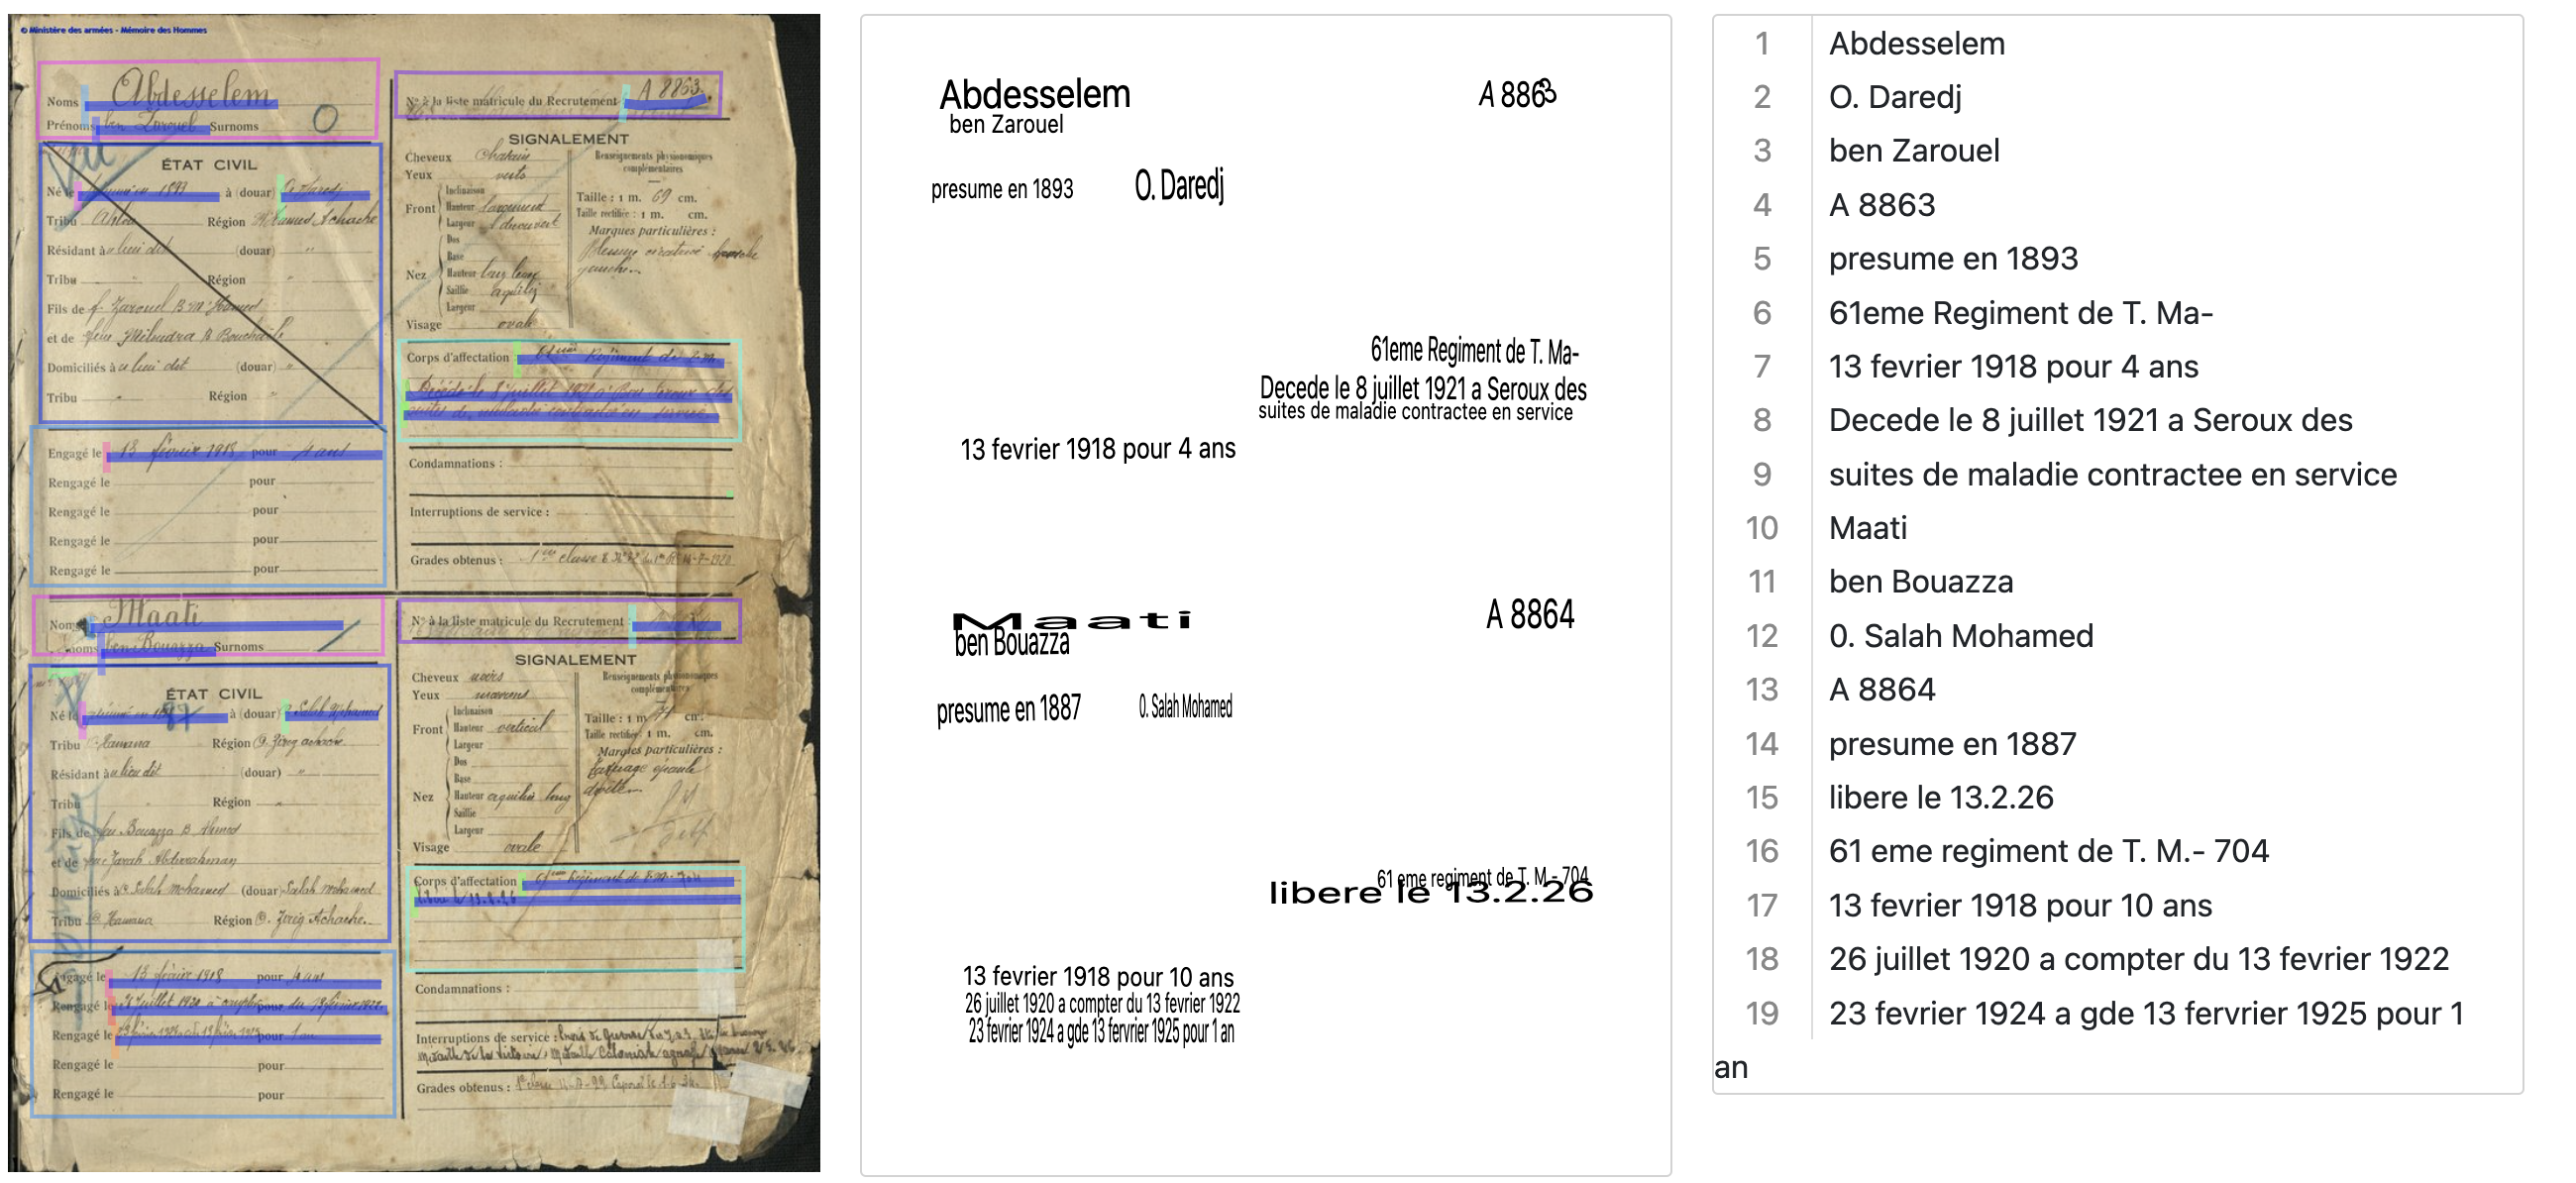
\includegraphics[scale=0.43]{Images/seg.png}
    \caption{Entrainement d'une transcription de matricule Marocain}
    \label{fig:Segmat}
\end{figure}
Ma méthode de segmentation a consisté à créer des régions dans le registre telles que l’état civil, le parcours individuel, le corps d’affection. À l'intérieur de ces régions, j’ai segmenté des lignes spécifiques comme le nom, ou le lieu de naissance. Cette méthode m'a permis d’obtenir des sorties en ALTO qui étaient organisées par contenu. Les fiches matricules originales se trouvent dans le dossier: transcription de mon github. Une fois les transcriptions terminées, j’ai traité ce dossier avec XSLT pour le transformer en XML et ensuite en csv. Avec ces informations stockées dans des fichiers csv, on peut envisager une analyse beaucoup plus claire et puissante des registres matricules. Le but de cet exercice était de me familiariser avec les méthodes de l’HTR afin de préparer le travail d'échantillonnage, de modélisation et de transcription pour l'année prochaine.   
  

\section{Conclusion}
Mon travail de méthodologie de cette année me permet d’avoir un aperçu des résultats que je pourrais obtenir après une étude plus complète. En même temps, il représente une première étape importante dans ma méthodologie, étant donné le manque de conseils reçus sur le plan quantitatif et l'étendue de mes sources qualitatives à traiter. Comme il sera expliqué dans la section suivante, cette étape m'a permis d'effectuer une vérification préliminaire de mes résultats avec d'autres travaux historiques.
